% Questo è il mio primo documento serio scritto in Latex, quindi potrebbe contenere degli orrori
% Chiedo umilmente scusa xD
\documentclass[a4paper, titlepage]{article}
\usepackage[italian]{babel}
\usepackage[utf8]{inputenc}
\usepackage{hyperref}
\usepackage{amsmath}
\usepackage{amssymb}
\usepackage{mathtools}
\hypersetup{
	colorlinks,
	citecolor=black,
	filecolor=black,
	linkcolor=black,
	urlcolor=black
}
\usepackage{tikz}
\usetikzlibrary{arrows}
\usepackage{pgfplots}

%opening
\title{Elaborazione di Segnali e Immagini}
\author{Matteo Iervasi}
\date{ }

\begin{document}

\maketitle

\newpage
	\tableofcontents
\newpage

\section{Introduzione}
\subsection{Che cos'è un segnale?}
Si definisce \textbf{segnale} una qualsiasi grandezza fisica che varia nel tempo e trasporta informazione. 
In generale esistono diversi tipi di segnali, ma in natura sono quasi sempre casuali e continui.

Una prima grossa suddivisione della teoria dei segnali si basa sul tipo di segnale: i segnali \textbf{deterministici}, 
di cui è possibile predire il valore in un qualunque istante a piacere, e i segnali \textbf{stocastici} o \textbf{aleatori}, 
il cui valore non è prevedibile, ma su cui è possibile ottenere soltanto delle proprietà statistiche.
Altra suddivisione è quella in segnali \textbf{continui} e \textbf{discreti}, ai quali si associano rispettivamente le comunicazioni \textit{analogiche} e le comunicazioni \textit{digitali}.

Parte della teoria dei segnali è profondamente connessa con la \textbf{teoria dei sistemi}, in quanto molti segnali transitano come input 
in sistemi che elaborano ovvero trasformano il segnale in ingresso restituendo in uscita un certo output.

\subsection{Che cos'è un sistema?}
Possiamo definire un \textbf{sistema} (dinamico) come un modello matematico che rappresenta un oggetto che evolve nel tempo.
\begin{figure}[h]
	\centering
	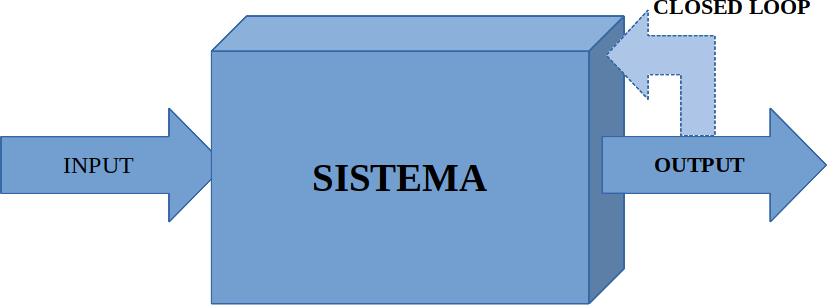
\includegraphics[width=0.7\linewidth]{img/sistema}
	\caption[Schema di un sistema]{Schema di un sistema}
	\label{fig:sistema}
\end{figure}

\subsection{Classificazione dei segnali}
Come accennato prima, possiamo suddividere i segnali in diverse categorie:
\begin{itemize}
	\item Analogici - Digitali
	\item Continui nel tempo - Discreti nel tempo
	\item Periodici - Aperiodici
	\item Deterministici - Casuali
	\item Segnali di energia - Segnali di potenza
	\item ...
\end{itemize}
È importante notare come le suddivisioni sopra elencate non siano esclusive tra loro, ci sono ad esempio segnali di potenza periodici, analogici e casuali, ecc.

\subsubsection{Segnali a tempo continuo e a tempo discreto}
Un segnale si definisce \textbf{a tempo continuo} quando il suo dominio ha la stessa cardinalità dei numeri reali, ed è quindi specificato per ogni reale.

\begin{tikzpicture}
	\begin{axis}[
		axis lines=left,
		xlabel=Tempo,
		ylabel=Ampiezza,
		trig format plots=rad,
	]
	\addplot[
		domain=0:4*pi,
		samples=360,
		color=blue,
		line width=1.25pt,
	]{sin(x)};
	\end{axis}
\end{tikzpicture}

Un segnale si definisce \textbf{discreto} quando il suo dominio ha la stessa cardinalità dei numeri naturali, ed è quindi specificato per valori discreti.

\begin{tikzpicture}
	\begin{axis}[
		axis lines=left,
		xlabel=Tempo,
		ylabel=Ampiezza,
		trig format plots=rad,
	]
	\addplot[
		domain=0:4*pi,
		samples=360,
		color=blue,
		line width=1.25pt,
		loosely dotted,
		line cap=round,
		]{sin(x)};
	\end{axis}
\end{tikzpicture}

\subsubsection{Segnali analogici e digitali}
Se parlando del dominio abbiamo i segnali a tempo continuo e a tempo discreto, possiamo distinguere i segnali analogici e digitali guardando i valori assunti dal codominio.
Quando l'ampiezza di un segnale può assumere qualsiasi valore in un intervallo continuo, parliamo di \textbf{segnale analogico}, viceversa quando assume solo un insieme
finito di valori parliamo di \textbf{segnale digitale}. In quest'ultimo caso il segnale si dice "\textit{quantizzato}".

\begin{tikzpicture}
	\begin{axis}[
		scale only axis,
		height=5cm,
		width=9cm,
		axis lines=left,
		xlabel=Tempo,
		ylabel=Ampiezza,
		trig format plots=rad,
	]
	\addplot[
		domain=0:8*pi,
		samples=360,
		color=blue,
		line width=1.25pt,
	]{sin(x)};
	\addlegendentry{Segnale analogico}
	\addplot+[
		color=red,
		mark=none,
		const plot,
		line width=1.25pt,
	]
	coordinates {
		(0,0.00)
		(1,0.84)
		(2,0.91)
		(3,0.14)
		(4,-0.76)
		(5,-0.96)
		(6,-0.28)
		(7,0.66)
		(8,0.99)
		(9,0.41)
		(10,-0.54)
		(11,-1.00)
		(12,-0.54)
		(13,0.42)
		(14,0.99)
		(15,0.65)
		(16,-0.29)
		(17,-0.96)
		(18,-0.75)
		(19,0.15)
		(20,0.91)
		(21,0.84)
		(22,-0.01)
		(23,-0.85)
		(24,-0.91)
	};
	\addlegendentry{Segnale digitale}
	\end{axis}
\end{tikzpicture}

\subsubsection{Segnali periodici e aperiodici}
Un segnale è periodico se esiste una costante positiva $T_{0}$ tale che
$$
	f(t+T_{0})=f(t) \qquad \forall t
$$
Il più piccolo valore di $T_{0}$ che soddisfa questa relazione è chiamato \textbf{periodo} della funzione. Un segnale periodico rimane invariato quando viene spostato
nel tempo.

\subsubsection{Segnali causali e non causali}
I segnali \textbf{causali} assumono il valore $0$ per $x<0$, viceversa i segnali \textbf{anti-causali} valgono $0$ per $x\geq0$.
I segnali \textbf{non causali} sono segnali il cui valore è diverso da $0$ da ambo i lati.

\subsubsection{Segnali pari e dispari}
Un segnale \textbf{pari} è un qualsiasi segnale $f$ tale che $f(t)=f(-t)$. Questi segnali sono facilmente riconoscibili in quanto simmetrici rispetto all'asse delle ordinate.
Un segnale \textbf{dispari} invece segue la relazione $f(t)=-f(-t)$.

\begin{center}
	\begin{tikzpicture}
	\begin{axis}[
		axis lines=center,
	]
	\addplot[
		color=blue,
		line width=1.25pt,
	]{5*x^2};
	\addlegendentry{Segnale pari};
	\addplot[
		color=red,
		line width=1.25pt,
	]{x^3};
	\addlegendentry{Segnale dispari};
	\end{axis}
\end{tikzpicture}
\end{center}

Qualsiasi segnale può essere riscritto come composizione di segnali pari e dispari:
\begin{align*}
	f(t)&=\dfrac{1}{2}(f(t)+f(-t))+\dfrac{1}{2}(f(t)-f(-t)) \\
	f_{e}(t)&=\dfrac{1}{2}(f(t)+f(-t)) \qquad \text{even component} \\
	f_{o}(t)&=\dfrac{1}{2}(f(t)-f(-t)) \qquad \text{odd component} \\
	f(t)&=f_{e}(t)+f_{o}(t)
\end{align*}

Alcune proprietà delle funzioni pari e dispari:
\begin{itemize}
	\item Funzione pari $\times$ Funzione dispari = Funzione dispari
	\item Funzione dispari $\times$ Funzione dispari = Funzione pari
	\item Funzione pari $\times$ Funzione pari = Funzione pari
	\item Area di una funzione pari:\\
	$\int_{-a}^{a} f_{e}(t) dt = 2\int_{0}^{a} f_{e}(t) dt$
	\item Area di una funzione dispari:\\
	$\int_{-a}^{a} f_{o}(t) dt = 0$
\end{itemize}

\subsubsection{Segnali deterministici e probabilistici}
Un segnale \textbf{deterministico} è un segnale la cui \textit{descrizione fisica} è nota a priori, per cui è possibile prevedere in ogni istante il valore del segnale mediante una formula matematica,
una regola o una tabella.
Per questo motivo è anche possibile calcolare i valori futuri dai valori passati senza alcuna incertezza sui valori di ampiezza.

\begin{center}
	\begin{tikzpicture}
	\begin{axis}[xlabel=Tempo,ylabel=Ampiezza]
	\addplot {cos(deg(x))+ln(x)};
	\addlegendentry{$cos(x)+ln(x)$}
	\end{axis}
	\end{tikzpicture}
\end{center}

Un segnale \textbf{probabilistico} invece è un segnale i cui valori di ampiezza non possono essere previsti con precisione, ma per i quali è solo possibile descrivere una probabilità, spesso basandosi
sulla media di altri valori.

\begin{center}
	\begin{tikzpicture}
	\begin{axis}[xlabel=Tempo,ylabel=Ampiezza]
	\addplot+[
	color=red,
	line width=1.25pt,
	]
	coordinates {
		(0,4)
		(1,7)
		(2,12)
		(3,19)
		(4,17)
		(5,9)
		(6,14)
		(7,12)
		(8,3)
		(9,4)
		(10,15)
		(11,16)
		(12,16)
		(13,17)
		(14,12)
		(15,9)
		(16,3)
		(17,11)
		(18,20)
		(19,9)
		(20,13)
		(21,15)
		(22,11)
		(23,15)
		(24,9)
	};
	\end{axis}
	\end{tikzpicture}
\end{center}

\subsection{Caratteristiche dei segnali}
Si definisce segnale di \textbf{lunghezza finita} un segnale i cui valori sono diversi da $0$ per un intervallo \textit{finito} di valori della variabile indipendente.
\begin{align*}
	f=f(t), \quad \forall t:t_{1} \leq t \leq t_{2}\\
	\text{dove} \qquad t_{1} > -\infty, t_{2} < +\infty
\end{align*}

Si definisce segnale di \textbf{lunghezza infinita} un segnale i cui valori sono diversi da $0$ per un intervallo \textit{infinito} di valori della variabile indipendente.
$$
	f(t)=sin(\omega t)
$$

La \textbf{dimensione} di un segnale indica la larghezza o la forza di esso. Useremo il concetto di \textit{norma} per quantificare questa nozione sia per segnali a tempo continuo che discreto.\\
L'area sotto la curva del segnale rappresenta \textbf{l'energia}.

\begin{center}
	\begin{tikzpicture}
	\begin{axis}[xlabel=Tempo,ylabel=Ampiezza,axis lines=left,]
	\addplot+[
	color=red,
	line width=1.25pt,
	mark=none,
	]
	coordinates {
		(0,0)
		(5,3)
		(5,0)
	};
	\end{axis}
	\end{tikzpicture}
\end{center}

L'\textbf{energia} di un segnale si calcola come:
$$
	E_{f} = \lim_{T\rightarrow\infty} \int_{-T/2}^{+T/2}|f(t)|^2dt
$$
Quando $0<E_{f}<+\infty$ il segnale è detto \textbf{di energia}.

La \textbf{potenza} di un segnale si calcola come:
$$
	P_{f} = \lim_{T\rightarrow\infty} \frac{1}{T} \int_{-T/2}^{+T/2}|f(t)|^2dt
$$
Quando $0<P_{f}<+\infty$ il segnale è detto \textbf{di potenza}.

La radice quadrata della potenza è detto \textbf{valore efficace}. Esso costituisce un parametro molto importante nella teoria dei segnali, alla base per esempio della definizione del \textbf{rapporto segnale/rumore}.
Possono esistere segnali per i quali né l'energia né la potenza sono finiti. Tuttavia nella pratica i segnali hanno energia finita, per cui sono segnali di energia 
(risulta impossibile generare un vero e proprio segnale di potenza, in quanto questo richiederebbe durata infinita ed energia infinita).

\subsection{Operazioni sui segnali}
\begin{itemize}
	\item \textbf{Spostamento}: Anticipo o ritardo di un segnale
	\begin{center}
		\begin{tikzpicture}
		\begin{axis}[xlabel=t,ylabel=f(t),axis lines=left,]
		\addplot[
		color=red,
		line width=1.25pt,
		mark=none,
		]
		coordinates {
			(0,0)
			(5,3)
			(7,0)
		};
		\addlegendentry{Originale};
		\addplot[
		color=blue,
		line width=1.25pt,
		mark=none,
		dashed,
		]
		coordinates {
			(-2,0)
			(3,3)
			(5,0)
		};
		\addlegendentry{Anticipato};
		\addplot[
		color=green,
		line width=1.25pt,
		mark=none,
		dashed,
		]
		coordinates {
			(2,0)
			(7,3)
			(9,0)
		};
		\addlegendentry{Ritardato};
		\end{axis}
		\end{tikzpicture}
	\end{center}
	\item \textbf{Scala}: Compressione o espansione di un segnale nel tempo
	\begin{center}
		\begin{tikzpicture}
		\begin{axis}[xlabel=t,ylabel=f(t),axis lines=left,]
		\addplot[
		color=red,
		line width=1.25pt,
		mark=none,
		]
		coordinates {
			(0,0)
			(5,3)
			(7,0)
		};
		\addlegendentry{Originale};
		\addplot[
		color=blue,
		line width=1.25pt,
		mark=none,
		dashed,
		]
		coordinates {
			(2,0)
			(5,3)
			(6,0)
		};
		\addlegendentry{Compresso};
		\addplot[
		color=green,
		line width=1.25pt,
		mark=none,
		dashed,
		]
		coordinates {
			(-2,0)
			(5,3)
			(9,0)
		};
		\addlegendentry{Espanso};
		\end{axis}
		\end{tikzpicture}
	\end{center}
	\item \textbf{Inversione}: Simmetria rispetto all'asse verticale
	\begin{center}
		\begin{tikzpicture}
		\begin{axis}[xlabel=t,ylabel=f(t),axis lines=left,]
		\addplot[
		color=red,
		line width=1.25pt,
		mark=none,
		]
		coordinates {
			(0,0)
			(5,3)
			(7,0)
		};
		\addlegendentry{Originale};
		\addplot[
		color=blue,
		line width=1.25pt,
		mark=none,
		dashed,
		]
		coordinates {
			(-0,0)
			(-5,3)
			(-7,0)
		};
		\addlegendentry{Inverso};
		\end{axis}
		\end{tikzpicture}
	\end{center}
\end{itemize}
\subsection{Funzioni utili}
\begin{itemize}
	\item Funzione gradino unitaria
	\begin{align*}
	u(t)=\left\{
		\begin{array}{ll}
		1 \quad t\geq0\\
		0 \quad t<0
		\end{array}
		\right.
	\end{align*}
	
	\item Funzione rampa unitaria
	\begin{align*}
	r(t)=\left\{
	\begin{array}{ll}
	0  \quad \text{if} \quad t<0\\
	\frac{t}{t_{0}} \quad  \text{if} \quad 0\leq t\leq t_{0}\\
	1 \quad \text{if} \quad t>t_{0}
	\end{array}
	\right.
	\end{align*}
	
	\item Impulso unitario
	\begin{align*}
	\delta(t)=0,t\neq0\\
	\int_{-\infty}^{+\infty}\delta(t)dt=1
	\end{align*}
	
	\item Funzione esponenziale
	$$f(t)=Ae^{j\omega t}$$
\end{itemize}
Di seguito elenchiamo alcune delle proprietà fondamentali della funzione \textit{impulso unitario}.
\begin{itemize}
	\item Moltiplicazione di una funzione per l'impulso
	\begin{align*}
	\phi(t)\delta(t)&=\phi(0)\delta(t)\\
	\phi(t)\delta(t-T)&=\phi(T)\delta(t-T)
	\end{align*}
	
	\item Proprietà del campionamento
	\begin{align*}
	&\int_{-\infty}^{+\infty} \phi(t)\delta(t)dt=\int_{-\infty}^{+\infty} \phi(0)\delta(t)dt=\phi(0)\int_{-\infty}^{+\infty} \delta(t)dt=\phi(0)\\
	&\int_{-\infty}^{+\infty} \phi(t)\delta(t-T)dt=\phi(T)
	\end{align*}
	L'area sotto la curva ottenuta dal prodotto dell'impulso traslato di T e la funzione $\varphi(t)$ è il valore ottenuto dalla funzione $\varphi(t)$ per $t=T$
	
	\item L'integrale dell'impulso è la funzione gradino
	\begin{align*}
		&\frac{du}{dt}=\delta(t)\\
		&\int_{-\infty}^{t}\delta(t)dt=u(t)\\
		&\text{Quindi}\\
		&\int_{-\infty}^{t}\delta(t)dt=u(t)=
		\left\{
		\begin{array}{ll}
		1 \quad t<0\\
		0 \quad t\geq0
		\end{array}
		\right.
	\end{align*}
\end{itemize}

\subsection{Sistemi lineari}
Un sistema è caratterizzato da \textbf{input}, \textbf{output} e da un \textbf{modello matematico} del sistema. L'\textbf{analisi} di un sistema prevede di determinare l'output di un sistema dato l'input, mentre l'operazione inversa è la \textbf{sintesi} o \textbf{progettazione}.

Come per i segnali, anche i sistemi possono essere classificati in varie categorie:
\begin{itemize}
	\item Lineari - Non lineari
	\item A parametri costanti - Parametri che cambiano nel tempo
	\item Istantanei (senza memoria) - Dinamici (con memoria)
	\item Causali - Non causali
	\item A tempo continuo - A tempo discreto
	\item Analogici - Digitali
	\item ...
\end{itemize}

\subsubsection{Proprietà dei sistemi lineari}
Elenchiamo di seguito alcune proprietà dei sistemi lineari:
\begin{itemize}
	\item \textbf{Additività}\\
	$f_{1} \rightarrow y_{1}$ e $f_{2} \rightarrow y_{2}$ allora $f_{1} +f_{2} \rightarrow y_{1}+y_{2}$
	\item \textbf{Omogeneità}\\
	$f_{1} \rightarrow y_{1}$ allora $a_{1} \times f_{1}\rightarrow a_{1}\times y_{1}$
	\item \textbf{Sovrapposizione}\\
	$a_{1} \times f_{1} + a_{2}\times f_{2} \rightarrow a_{1}\times y_{1}+a_{2}\times y_{2}$
\end{itemize}

\subsubsection{Risposta libera e risposta forzata}
La \textbf{risposta libera} di un sistema è la sua risposta quando l'ingresso è nullo.
L'output di un sistema per $t\geq0$ è il risultato di due cause indipendenti: le \textbf{condizioni iniziali} del sistema al tempo $t=0$ e l'input $f(t)$ per $t\geq0$.
Grazie alla \textit{linearità} la risposta totale del sistema è la \textbf{somma} della risposta libera e della risposta forzata.
Nella realtà abbiamo sistemi che sono lineari solo \textit{localmente}, che in genere rispondo linearmente a piccoli segnali e non linearmente a grandi segnali.
\begin{center}
	\begin{tikzpicture}
	\begin{axis}[xlabel=f,ylabel=y,axis lines=left,]
	\addplot[
	color=red,
	line width=1.25pt,
	]{x+2};
	\addlegendentry{Causale, lineare};
	\addplot[
	color=blue,
	line width=1.25pt,
	domain=-10:-4
	]{x+2};	
	\addplot[
	color=blue,
	line width=1.25pt,
	domain=-4:4,
	]{x^2+10*x+22};
	\addlegendentry{Causale, non lineare};
	\end{axis}
	\end{tikzpicture}
\end{center}

I sistemi i cui parametri \textit{non} cambiano nel tempo vengono detti \textbf{tempo invarianti}.
Per questi sistemi se l'input viene ritardato di $T$ secondi, l'output rimane identico a prima, ma ritardato di $T$.

I sistemi \textbf{istantanei} (senza memoria) sono quelli in cui l'output al tempo $t$ dipende esclusivamente dall'input al tempo $t$.
Se l'output dipende dagli eventi passati, il sistema viene definito \textbf{dinamico} (un sistema con memoria).
Un sottogruppo dei sistemi dinamici sono i sistemi con \textbf{memoria finita}, per i quali l'output al tempo $t$ è completamente determinato
dai segnali in input per gli ultimi $T$ istanti (il sistema ha quindi una memoria di capacità massima $T$).

\section{Analisi dei sistemi a tempo continuo}
Quando si studia un sistema, uno degli scopi più comuni è ricostruire le equazioni che lo regolano, permettendoci quindi di calcolare l'output del sistema dato un preciso input.
Uno degli strumenti fondamentali per questo scopo è la \textbf{risposta impulsiva} del sistema, che caratterizza completamente il comportamento di un sistema lineare tempo invariante.

Per il calcolo della risposta impulsiva ci serve prima la \textbf{risposta libera}.
Ricordiamo che trattandosi di sistemi lineari, valgono le proprietà di \textit{additività}, \textit{omogeneità} e \textit{sovrapposizione}.

Un sistema lineare tempo invariante (LTI) può essere descritto da un'equazione differenziale:
\[a_n\frac{d^nv(t)}{dt^n} + \ldots + a_1\frac{dv(t)}{dt} + a_0v(t) = b_m\frac{d^mu(t)}{dt^m} + \ldots + b_1\frac{du(t)}{dt} + b_0u(t),\]
in forma compatta
\begin{equation*}
	\sum_{i=0}^{n}a_i\frac{d^iv(t)}{dt^i} = \sum_{j=0}^{m}b_j\frac{d^ju(t)}{dt^j}
\end{equation*}
Nella pratica, $m$ è sempre minore di $n$.

\subsection{Calcolo della risposta libera}
Nella teoria dei sistemi dinamici, la \textbf{risposta libera} o risposta ad ingresso nullo di un sistema dinamico, anche detta ‘‘risposta libera nello stato’’ in quanto interessa le variabili di stato del sistema,
è la sua risposta quando l'ingresso è nullo, in modo che il comportamento del sistema dipende soltanto dalle condizioni iniziali.
Nei sistemi lineari il principio di sovrapposizione stabilisce in particolare che è possibile scomporre l'uscita come la somma della risposta libera più la risposta forzata, quindi possiamo dividere il segnale di uscita $v(t)$ come:
\[
v(t)=
\begin{cases}
	u(t) \ne 0, c.i. = 0\\
	u(t) = 0, c.i. \ne 0
\end{cases}
\]
La risposta libera si calcola come:
\begin{equation*}
	\sum_{i=0}^{n}a_i\frac{d^iv(t)}{dt^i}=0
\end{equation*}
All'equazione differenziale omogenea associamo un’equazione algebrica detta \textbf{equazione caratteristica} del sistema:
\begin{equation*}
	\sum_{i=0}^{n}a_is^i=0, \quad s \in C
\end{equation*}
Se $\lambda_1,...,\lambda_r$ sono le $r\leq n$ soluzioni distinte dell'equazione caratteristica, e $\mu_1,....,\mu_r \in \mathbb{N}$ rappresentano le rispettive molteplicità, ogni soluzione dell'omogenea, in particolare la risposta libera, può essere espressa nella forma:
\begin{equation*}
	v_l(t)=\sum_{i=1}^{r}\sum_{l=0}^{\mu_i-1}c_{i,l}e^{\lambda_it}\frac{t^l}{l!}
\end{equation*}
per opportuni $c_{i,l} \in \mathbb{C}$. Le soluzioni dell'omogenea del tipo $e^{\lambda_it}\frac{t^l}{l!}, t \in \mathbb{R}$, vengono dette \textbf{modi naturali}.

\subsection{Calcolo della risposta impulsiva}
La risposta impulsiva di un sistema è la sua uscita quando è soggetto ad un ingresso a \textbf{delta di Dirac};
viene utilizzata per descrivere la \textbf{risposta in frequenza} di un sistema dinamico ad una perturbazione generica.
La delta di Dirac vista come ‘‘funzione’’ contiene equamente tutte le frequenze, e si presta particolarmente bene allo studio teorico nel dominio della frequenza di un sistema lineare.

Il comportamento ingresso-uscita di un sistema dinamico lineare stazionario (LTI) è completamente caratterizzato dalla sua risposta impulsiva, la cui trasformata di Laplace viene detta funzione di trasferimento del sistema LTI.

La risposta impulsiva, che denoteremo con $h(t)$, si calcola come:
$$ h(t)=d_0\delta(t)+\left(\sum_{i=1}^{r} \sum_{l=0}^{\mu_i-1} d_{i,l}e^{\lambda_it}\frac{t^l}{l!}\right)\delta_{-1}(t) $$

Notiamo che la risposta impulsiva contiene la risposta libera, ovvero tutti i modi naturali del sistema dopo l'impulso. Il termine $d_0\delta(t)$ è non nullo se $m=n$ e indica il termine impulsivo.
La risposta libera viene moltiplicata per la funzione gradino in modo da "tagliare" tutto ciò che c'era prima di $t=0$ e garantire che le c.i. a $t=0^-$ siano nulle.

\subsection{Integrale di convoluzione}
Date le funzioni $v_1(t)$ e $v_2(t)$, con $t\in \mathbb{R}$, definiamo \textbf{integrale di convoluzione} di $v_1$ e $v_2$ la funzione definita come:
\begin{equation*}
	[v_1]
\end{equation*}

\end{document}
